\documentclass[11pt,a4paper]{article}

% ============ PAQUETES ============
\usepackage[utf8]{inputenc}
\usepackage[T1]{fontenc}
\usepackage{amsmath, amssymb}
\usepackage{graphicx}
\usepackage{geometry}
\usepackage{tikz}
\usetikzlibrary{positioning}
\usepackage{booktabs}
\usepackage{array}
\usepackage{enumitem}
\usepackage{hyperref}
\usepackage{algorithm}
\usepackage{algpseudocode}
\usepackage{xcolor}
\usepackage{fancyhdr}
\usepackage{listings}
\usepackage{tocloft}

% Nota: el paquete babel con idioma espanol no esta disponible en el
% entorno de compilacion usado para preparar este documento (no hay
% acceso para instalar texlive-lang-spanish). Se traducen a mano las
% pocas cadenas automaticas usadas (Resumen, Indice). Si se recompila
% en Overleaf o con una instalacion completa de TeX Live, puede
% agregarse \usepackage[spanish]{babel} sin que cambie el contenido.
\renewcommand{\abstractname}{Resumen}
\renewcommand{\contentsname}{Índice}

\geometry{margin=2.5cm}
\hypersetup{colorlinks=true, linkcolor=blue, urlcolor=blue, citecolor=blue}

\pagestyle{fancy}
\fancyhf{}
\lhead{Algoritmos Avanzados -- Informe, Primera Entrega}
\rhead{Grupo 1 -- Cobertura de Vértices}
\cfoot{\thepage}

\lstset{
	basicstyle=\ttfamily\small,
	breaklines=true,
	frame=single,
	columns=fullflexible,
	backgroundcolor=\color{gray!8}
}

% ============ DATOS DEL PROYECTO ============
\title{
	\vspace{-1cm}
	\textbf{Optimización de la Ubicación de Sistemas de Detección de Intrusos \\
	mediante Cobertura de Vértices} \\
	\large Comparación experimental entre una heurística greedy por grado y una
	2-aproximación por emparejamiento maximal
}
\author{
	Grupo 1 \\
	\small Universidad Nacional de San Antonio Abad del Cusco \\
	\small Escuela Profesional de Ingeniería Informática y de Sistemas \\
	\small Asignatura: Algoritmos Avanzados \\
	\small Docente: Héctor Eduardo Ugarte Rojas \\
	\small Atributo del graduado evaluado: AG\_C06 -- Aprendizaje a lo largo de la vida
}
\date{Semestre académico 2026-2 \\ Informe de la Primera Entrega (Avances 1, 2 y 3)}

\begin{document}

\maketitle
\thispagestyle{fancy}

\begin{abstract}
\noindent
Este informe documenta el estado del proyecto grupal sobre \textbf{Cobertura de Vértices
(Vertex Cover)} al cierre de la Primera Entrega, integrando los tres avances presentados
durante el periodo (formulación del problema, diseño algorítmico con plan de validación, y
prototipo mínimo ejecutable). El problema se aplica al contexto de ciberseguridad y
monitoreo de redes: ubicar sistemas de detección de intrusos (IDS) en el número mínimo de
routers tal que todo enlace de la red quede monitoreado por al menos uno de sus extremos.
Se implementaron y compararon tres estrategias algorítmicas -- una heurística greedy por
grado, una 2-aproximación por emparejamiento maximal con garantía matemática demostrable, y
una solución exacta de referencia por fuerza bruta -- sobre un sistema reproducible, versionado
en Git, con 27 pruebas automatizadas (casos básicos, límite y adversarios) y un primer
experimento comparativo. El hallazgo más relevante del periodo fue un defecto de
no-determinismo en la implementación inicial (dependiente del orden de iteración de los
conjuntos de Python), detectado mediante las propias pruebas y corregido antes del cierre
de la entrega, documentado aquí como evidencia de aprendizaje autónomo y pensamiento
crítico. Los resultados preliminares muestran que el greedy iguala al óptimo en la mayoría
de las instancias de prueba, mientras que el matching maximal se mantiene siempre dentro de
su cota teórica de $2\times$ el óptimo; el algoritmo exacto confirma un crecimiento
exponencial del tiempo de ejecución ya visible en instancias de menos de 20 vértices. El
informe cierra señalando explícitamente lo pendiente para la Entrega 2: un solver exacto
escalable por programación lineal entera, una metodología experimental ampliada y la
optimización de la complejidad del algoritmo greedy.
\end{abstract}

\tableofcontents
\thispagestyle{fancy}
\newpage

% ======================================================
\section{Resumen}

Ver el Resumen en la primera página. Esta sección numerada se incluye para respetar el
índice de contenidos exigido por la guía del proyecto (\emph{Contenidos del informe final},
ítem 1); su contenido es el mismo abstract presentado arriba, ya que en esta primera
entrega no hay una sección separada que condense el documento con un alcance distinto.

% ======================================================
\section{Introducción}

\subsection{Contexto y motivación}
En una red de comunicaciones, cada enlace físico entre dispositivos (routers, switches) es
un punto potencial de tráfico malicioso o de fallas. Instalar un sistema de detección de
intrusos (IDS) o firewall en \emph{todos} los routers de la red garantiza visibilidad
completa del tráfico, pero resulta costoso e innecesario en equipos, licencias y
mantenimiento. Basta con que cada enlace tenga \emph{al menos uno} de sus dos extremos
monitoreado para que el tráfico que circula por él pueda inspeccionarse. Este planteamiento
corresponde exactamente al problema clásico de \textbf{Cobertura de Vértices (Vertex
Cover)}: dado un grafo no dirigido, encontrar el subconjunto mínimo de vértices tal que toda
arista tenga al menos un extremo en dicho subconjunto.

\subsection{El problema}
Vertex Cover es NP-difícil en su formulación general \cite{karp1972}, por lo que no se
conoce (ni se espera encontrar, bajo la conjetura $P \neq NP$) un algoritmo que resuelva
todas las instancias de forma óptima en tiempo polinomial. Esto hace que el problema sea un
caso de estudio natural para \textbf{comparar estrategias}: algoritmos exactos (correctos
pero costosos), heurísticos (rápidos pero sin garantía) y de aproximación con cota
demostrable (rápidos y con garantía parcial). Esa comparación -- no la implementación de un
único algoritmo -- es el eje central exigido por la línea de trabajo asignada al grupo
("cobertura de vértices y comparación de estrategias de aproximación").

\subsection{Objetivos}

\subsubsection*{Objetivo general}
Desarrollar y evaluar experimentalmente una solución computacional para el problema de
Cobertura de Vértices aplicado a la ubicación de sistemas de monitoreo en redes,
demostrando aprendizaje autónomo, adaptación a herramientas pertinentes y pensamiento
crítico en la selección, implementación y análisis de alternativas algorítmicas.

\subsubsection*{Objetivos específicos}
\begin{enumerate}[itemsep=2pt]
	\item Formular el problema mediante entradas, salidas, restricciones, supuestos y
	función objetivo claramente definidos (Avance 1).
	\item Diseñar la arquitectura del sistema (módulos, estructuras de datos, formatos de
	archivo) y documentar el pseudocódigo y análisis de complejidad de cada algoritmo
	(Avance 2).
	\item Implementar al menos dos algoritmos comparables -- se implementaron tres -- y un
	mecanismo de referencia exacto para validar instancias pequeñas.
	\item Diseñar y ejecutar un plan de pruebas que cubra casos básicos, límite y
	adversarios, con un criterio de verificación explícito de las salidas.
	\item Construir un prototipo mínimo ejecutable, demostrable en vivo con una instancia
	conocida o una propuesta en el momento (Avance 3).
	\item Diseñar experimentos reproducibles que comparen tiempo de ejecución y calidad de
	solución (ratio de aproximación empírico) entre los algoritmos.
	\item Evaluar críticamente las herramientas candidatas, los resultados obtenidos, los
	supuestos y las limitaciones del sistema actual.
	\item Documentar el proceso de aprendizaje autónomo del grupo a lo largo de las tres
	entregas progresivas.
\end{enumerate}

\subsection{Alcance de esta entrega}
Este informe cubre lo exigido para la \textbf{Primera Entrega}: formulación del problema,
diseño del sistema con su plan de validación, y un prototipo mínimo ejecutable con
resultados experimentales \emph{preliminares}. No incluye todavía: el solver exacto
escalable por programación lineal entera (ILP), la metodología experimental ampliada a
múltiples densidades y topologías, ni la defensa individual, que corresponden a la Entrega
2 y a la Entrega 3 respectivamente. Esto se señala explícitamente en cada sección donde
aplica, en vez de presentar resultados parciales como si fueran definitivos.

\subsection{Organización del documento}
La Sección~\ref{sec:fundamentos} presenta los fundamentos teóricos y el proceso de
aprendizaje autónomo del grupo. La Sección~\ref{sec:stack} evalúa y justifica el stack
tecnológico. La Sección~\ref{sec:formulacion} formula el problema formalmente. Las
Secciones~\ref{sec:diseno-algoritmico} y~\ref{sec:diseno-sistema} cubren el diseño
algorítmico y el diseño del sistema. La Sección~\ref{sec:pruebas} describe la estrategia de
pruebas. Las Secciones~\ref{sec:metodologia} y~\ref{sec:resultados} presentan la
metodología experimental y sus resultados. La Sección~\ref{sec:discusion} discute
críticamente esos resultados. La Sección~\ref{sec:conclusiones} cierra con conclusiones y
recomendaciones, seguida de referencias y anexos.

% ======================================================
\section{Fundamentos y aprendizaje autónomo}
\label{sec:fundamentos}

\subsection{Conceptos y algoritmos requeridos}
El desarrollo del proyecto requirió manejar con solvencia los siguientes conceptos:
\begin{itemize}
	\item \textbf{Teoría de grafos básica}: grafos no dirigidos, grado de un vértice,
	cobertura de vértices, y su relación de dualidad con \emph{Independent Set}
	($V \setminus C$ es un conjunto independiente si y solo si $C$ es una cobertura de
	vértices).
	\item \textbf{NP-completitud}: por qué Vertex Cover es NP-difícil \cite{karp1972}, y qué
	implica eso para la estrategia de solución (no buscar un algoritmo exacto polinomial,
	sino comparar heurísticas, aproximaciones y un exacto acotado en tamaño).
	\item \textbf{Algoritmos de aproximación}: qué es una garantía de aproximación de
	factor $k$, y cómo se demuestra formalmente (ver la demostración de la cota $2\times$ del
	matching maximal en la Sección~\ref{sec:diseno-algoritmico}) \cite{vazirani2003}.
	\item \textbf{Análisis de complejidad algorítmica}: notación $O(\cdot)$ para caracterizar
	el comportamiento de cada algoritmo en función de $|V|$ y $|E|$ \cite{clrs2009}.
\end{itemize}

\subsection{Fuentes estudiadas y criterios de selección}
Se priorizaron fuentes académicas y documentación oficial de las herramientas, siguiendo el
criterio explícito de la guía del proyecto (instrucción adicional 11: "se priorizarán
artículos, libros, documentación oficial y recursos técnicos verificables"):
\begin{itemize}
	\item Material de referencia sobre NP-completitud y algoritmos de aproximación
	(Cormen et al., \emph{Introduction to Algorithms} \cite{clrs2009}; Vazirani,
	\emph{Approximation Algorithms} \cite{vazirani2003}), elegidos por ser textos
	estándar y ampliamente citados en la literatura de algoritmos.
	\item Documentación oficial de \texttt{pytest}, \texttt{PuLP} y \texttt{NetworkX},
	priorizada sobre tutoriales de terceros por ser la fuente autoritativa y vigente de
	cada herramienta.
\end{itemize}

\subsection{Conocimientos nuevos que el grupo tuvo que adquirir}
\begin{itemize}
	\item La demostración formal de por qué el emparejamiento (\emph{matching}) maximal
	produce una cobertura de a lo sumo el doble del tamaño óptimo -- no bastaba con saber
	que el algoritmo existe, sino poder argumentar la cota.
	\item El comportamiento de la aleatorización de hash en Python (\texttt{PYTHONHASHSEED})
	y su efecto sobre el orden de iteración de un \texttt{set()}, que resultó ser la causa
	de un defecto de reproducibilidad real en la implementación (detallado en la
	Sección~\ref{sec:discusion}).
	\item Formulación de programación lineal entera (ILP) para Vertex Cover, como base para
	incorporar un solver escalable en la Entrega 2 (minimizar $\sum_v x_v$ sujeto a
	$x_u + x_v \geq 1$ para toda arista $(u,v)$, con $x_v \in \{0,1\}$).
	\item Uso de \texttt{pytest} con parametrización (\texttt{@pytest.mark.parametrize}) para
	repetir una misma verificación sobre múltiples instancias generadas aleatoriamente sin
	duplicar código de prueba.
\end{itemize}

\subsection{Estrategia y evidencias de aprendizaje autónomo}
El grupo mantiene una \textbf{bitácora de aprendizaje} (\texttt{docs/bitacora.md} en el
repositorio) con una entrada por sesión real de trabajo, registrando qué se hizo, qué se
tuvo que aprender o decidir por cuenta propia, y qué quedó pendiente. Esta bitácora es la
evidencia principal del indicador AG-C06.01 y respalda, con fecha y contexto, los hallazgos
que se resumen en este informe (en particular, el defecto de reproducibilidad de la
Sección~\ref{sec:discusion}, que se documentó en el momento en que se encontró, no de forma
retrospectiva). El Anexo~\ref{anexo:bitacora} reproduce un resumen de esa bitácora.

% ======================================================
\section{Evaluación y selección del stack tecnológico}
\label{sec:stack}

\subsection{Alternativas consideradas y criterios de comparación}
Se aplicaron cinco criterios generales a toda decisión tecnológica: (1) facilidad de
instalación sin dependencias del sistema operativo, (2) calidad y vigencia de la
documentación oficial, (3) curva de aprendizaje razonable para el tiempo disponible,
(4) adopción y soporte de la comunidad, y (5) que no añadiera complejidad innecesaria al
núcleo algorítmico (instrucción adicional 5 de la guía: "la interfaz es un medio de
interacción y no reemplaza el núcleo algorítmico").

\begin{center}
\begin{tabular}{p{2.9cm}p{4.8cm}p{6.5cm}}
	\toprule
	\textbf{Necesidad} & \textbf{Candidatas} & \textbf{Tecnología seleccionada y justificación} \\
	\midrule
	Lenguaje principal &
		Python 3 vs. Java vs. C++ &
		Python 3: sintaxis concisa para prototipado algorítmico, \texttt{set} y \texttt{dict}
		nativos adecuados para listas de adyacencia, y es la configuración de referencia
		sugerida por la guía del curso. \\
	Pruebas unitarias &
		\texttt{pytest} vs. \texttt{unittest} (estándar) &
		\texttt{pytest}: sintaxis de \texttt{assert} plano (más legible), soporte nativo de
		parametrización, amplia adopción y documentación. \\
	Manejo y visualización de grafos &
		\texttt{NetworkX} vs. implementación propia pura &
		Implementación propia para el núcleo (control total sobre la complejidad, requisito
		pedagógico del curso); \texttt{NetworkX} queda como candidata para visualización en
		la Entrega 2. \\
	Solver exacto escalable &
		\texttt{PuLP} vs. \texttt{OR-Tools} &
		\texttt{PuLP} (tecnología emergente del proyecto, pendiente de completar en la
		Entrega 2): instala el solver CBC junto con el paquete, sin dependencias del
		sistema; API declarativa simple para la formulación ILP estándar de Vertex Cover.
		\texttt{OR-Tools} se descarta por ahora por una curva de aprendizaje mayor frente al
		beneficio adicional en instancias de este tamaño. \\
	Datos y gráficos &
		\texttt{pandas} + \texttt{matplotlib} &
		Estándar de facto, documentación extensa, suficiente para el volumen de datos de
		este proyecto. \\
	Control de versiones &
		Git + GitHub &
		Exigido por la guía del proyecto (instrucción adicional 3); historial de commits
		como evidencia de evolución real del trabajo. \\
	Documentación &
		\LaTeX{} + Markdown &
		\LaTeX{} para los documentos formales de cada entrega (control tipográfico de
		fórmulas, pseudocódigo y tablas); Markdown para la bitácora y notas operativas,
		por ser más rápido de editar y de revisar en diffs de Git. \\
	\bottomrule
\end{tabular}
\end{center}

\subsection{Procedimiento de aprendizaje e integración}
El flujo seguido para cada herramienta nueva fue: (1) leer la documentación oficial de
inicio rápido, (2) escribir un script mínimo de prueba fuera del proyecto para confirmar el
comportamiento esperado, (3) integrarla al proyecto real, y (4) cubrirla con al menos una
prueba automatizada. Este procedimiento se siguió explícitamente para \texttt{pytest} (su
sintaxis de parametrización se validó primero en un archivo de prueba aislado antes de
usarse en \texttt{tests/test\_solver.py}).

\subsection{Dificultades de adopción y soluciones aplicadas}
La dificultad de adopción más significativa del periodo no fue con una biblioteca externa,
sino con el propio lenguaje: el comportamiento no determinístico de la iteración sobre
\texttt{set()} en Python (detallado como hallazgo central en la Sección~\ref{sec:discusion}).
Una segunda dificultad, menor, fue la imposibilidad de instalar el paquete de idioma
español de \LaTeX{} (\texttt{babel-spanish}) en el entorno de compilación usado para
preparar los documentos de las tres entregas, sin acceso a instalarlo; se resolvió
prescindiendo de \texttt{babel} y ajustando a mano los puntos donde la falta de guionado en
español causaba desbordes de texto en tablas, priorizando -- de nuevo según la instrucción
adicional 5 -- no bloquear la entrega por una herramienta no esencial al núcleo del
proyecto.

% ======================================================
\section{Formulación del problema}
\label{sec:formulacion}

\subsection{Modelo}
La topología de la red se representa como un grafo no dirigido $G = (V, E)$, donde:
\begin{itemize}
	\item $V$ es el conjunto de routers/switches de la red.
	\item $E$ es el conjunto de enlaces físicos entre dichos dispositivos.
\end{itemize}

\subsection{Entradas}
\begin{itemize}
	\item Un grafo $G = (V, E)$ que representa la topología de la red, en formato JSON
	(ver Sección~\ref{sec:diseno-sistema}).
	\item (Extensión futura, no implementada en esta entrega) costo de instalación por nodo,
	para una variante ponderada del problema.
\end{itemize}

\subsection{Salidas}
\begin{itemize}
	\item Un subconjunto $C \subseteq V$: los routers donde se instalará el sistema de
	monitoreo.
	\item El tamaño $|C|$ obtenido por cada algoritmo, para fines comparativos.
	\item Verificación booleana de que $C$ es una cobertura válida de $E$.
\end{itemize}

\subsection{Restricciones}
\begin{itemize}
	\item Para toda arista $(u,v) \in E$ debe cumplirse $u \in C \lor v \in C$.
	\item $C \subseteq V$.
\end{itemize}

\subsection{Supuestos}
\begin{itemize}
	\item La topología de la red es estática durante el cálculo de la solución.
	\item El grafo es no dirigido y no ponderado en esta primera fase del proyecto.
	\item Un router monitoreado detecta el tráfico de \emph{todos} sus enlaces directos.
\end{itemize}

\subsection{Función objetivo}
\begin{equation}
	\min_{C \subseteq V} |C|
	\quad \text{sujeto a} \quad
	\forall (u,v) \in E: \; u \in C \; \lor \; v \in C
\end{equation}

\subsection{Ejemplo: instancia pequeña resuelta manualmente}
\label{sec:ejemplo-manual}

Se usa una mini-red de 6 routers como ejemplo ilustrativo, resuelta primero a mano
(Avance 1) y luego reproducida con el sistema real (Sección~\ref{sec:resultados}):

\begin{center}
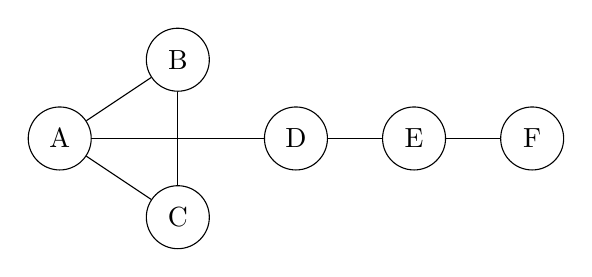
\begin{tikzpicture}[scale=1.0, every node/.style={circle, draw, minimum size=0.8cm}]
	\node (A) at (0,1)   {A};
	\node (B) at (1.5,2) {B};
	\node (C) at (1.5,0) {C};
	\node (D) at (3,1)   {D};
	\node (E) at (4.5,1) {E};
	\node (F) at (6,1)   {F};

	\draw (A) -- (B);
	\draw (A) -- (C);
	\draw (A) -- (D);
	\draw (B) -- (C);
	\draw (D) -- (E);
	\draw (E) -- (F);
\end{tikzpicture}
\end{center}

\[
V = \{A, B, C, D, E, F\}, \qquad
E = \{(A,B),(A,C),(A,D),(B,C),(D,E),(E,F)\}
\]

\textbf{Grados iniciales:} $\deg(A)=3,\ \deg(B)=2,\ \deg(C)=2,\ \deg(D)=2,\ \deg(E)=2,\ \deg(F)=1$.

\textbf{Greedy por grado:} se elige $A$ (grado 3), luego $E$ (grado 2 entre las aristas
restantes), luego $B$ (o $C$) para cubrir la arista $BC$ que queda pendiente.
$C_{\text{greedy}} = \{A, E, B\}$, $|C_{\text{greedy}}| = 3$.

\textbf{Matching maximal:} se toma arbitrariamente $(A,B)$, agregando ambos extremos y
eliminando todas las aristas que tocan a $A$ o $B$; de lo que queda se toma $(D,E)$,
agregando ambos extremos. $C_{\text{match}} = \{A, B, D, E\}$, $|C_{\text{match}}| = 4$.

\textbf{Óptimo de referencia (por inspección):} $C^{*} = \{A, C, E\}$ cubre las 6 aristas,
por lo tanto $|C^{*}| = 3$.

\begin{center}
\begin{tabular}{lccc}
	\toprule
	\textbf{Algoritmo} & \textbf{Cobertura} & \textbf{Tamaño} & \textbf{Respecto al óptimo (3)} \\
	\midrule
	Greedy por grado             & $\{A, B, E\}$    & 3 & Óptimo en esta instancia \\
	Matching maximal (2-aprox)   & $\{A, B, D, E\}$ & 4 & $1.33\times$ el óptimo \\
	Exacto (referencia)          & $\{A, C, E\}$    & 3 & --- \\
	\bottomrule
\end{tabular}
\end{center}

Este contraste -- heurística sin garantía formal pero buen desempeño práctico, frente a
aproximación con garantía matemática pero resultado subóptimo en casos concretos -- es el
eje de la comparación experimental desarrollada en este informe.

% ======================================================
\section{Diseño algorítmico}
\label{sec:diseno-algoritmico}

\subsection{Greedy por grado (\texttt{greedy\_degree\_vertex\_cover})}

\begin{algorithm}[H]
\caption{\texttt{greedy\_degree\_vertex\_cover}}
\begin{algorithmic}[1]
\State $E' \gets E$ \Comment{aristas pendientes}
\State $C \gets \emptyset$
\While{$E' \neq \emptyset$}
	\State calcular $\deg_{E'}(v)$ para cada $v$ incidente en $E'$
	\State $v^{*} \gets \arg\max_v \deg_{E'}(v)$
	\State $C \gets C \cup \{v^{*}\}$
	\State $E' \gets E' \setminus \{(u,w) \in E' : u = v^{*} \lor w = v^{*}\}$
\EndWhile
\State \Return $C$
\end{algorithmic}
\end{algorithm}

\textbf{Invariante de ciclo:} al inicio de cada iteración, $E'$ es exactamente el conjunto
de aristas de $E$ no cubiertas por $C$. Esto se cumple trivialmente al inicio ($C=\emptyset$,
$E'=E$) y se preserva en cada paso, porque al agregar $v^{*}$ a $C$ se eliminan de $E'$
exactamente las aristas que $v^{*}$ cubre y ninguna otra.

\textbf{Corrección:} el ciclo termina cuando $E' = \emptyset$, es decir, cuando toda arista
de $E$ tiene al menos un extremo en $C$ (por el invariante). Por lo tanto $C$ devuelto es
siempre una cobertura de vértices válida.

\textbf{Complejidad:} en la implementación actual (\texttt{src/solver.py}), cada iteración
recorre las aristas restantes para recalcular grados: $O(E)$ por iteración, hasta $O(V)$
iteraciones en el peor caso $\Rightarrow O(V \cdot E)$. Puede optimizarse a
$O((V+E)\log V)$ manteniendo una cola de prioridad; queda identificado como mejora
pendiente para la Entrega 2 (Sección~\ref{sec:conclusiones}).

\textbf{Garantía de aproximación:} ninguna cota fija demostrable en el peor caso general
(existen instancias donde el greedy se aleja más del óptimo que el matching maximal); en la
práctica, sobre las instancias probadas en este periodo, el ratio empírico se mantuvo entre
1.0x y 1.2x (Sección~\ref{sec:resultados}).

\subsection{Matching maximal / 2-aproximación (\texttt{maximal\_matching\_vertex\_cover})}

\begin{algorithm}[H]
\caption{\texttt{maximal\_matching\_vertex\_cover}}
\begin{algorithmic}[1]
\State $E' \gets E$
\State $C \gets \emptyset$
\While{$E' \neq \emptyset$}
	\State tomar $(u,v) \in E'$ \Comment{orden canónico, ver nota de reproducibilidad}
	\State $C \gets C \cup \{u, v\}$
	\State $E' \gets E' \setminus \{(a,b) \in E' : a \in \{u,v\} \lor b \in \{u,v\}\}$
\EndWhile
\State \Return $C$
\end{algorithmic}
\end{algorithm}

\textbf{Invariante:} las aristas elegidas en pasos sucesivos del ciclo
$(u_1,v_1), (u_2,v_2), \dots$ nunca comparten un extremo entre sí, porque cada elección
elimina de $E'$ todas las aristas incidentes a los dos vértices recién agregados antes de
la siguiente elección. Es decir, el conjunto de aristas elegidas forma siempre un
\emph{matching} (emparejamiento) del grafo.

\textbf{Corrección:} igual que en el greedy, el ciclo termina solo cuando $E' = \emptyset$,
así que $C$ cubre toda arista de $E$.

\textbf{Complejidad:} $O(V+E)$: cada arista se visita y se elimina a lo sumo una vez del
conjunto de pendientes.

\textbf{Demostración de la garantía de aproximación.} Sea $k$ el número de aristas elegidas
por el algoritmo (el tamaño del matching). Como esas $k$ aristas son disjuntas dos a dos
(invariante anterior), ningún vértice puede cubrir más de una de ellas. Por lo tanto,
\emph{toda} cobertura de vértices válida -- incluida la óptima $C^{*}$ -- debe contener al
menos un extremo distinto de cada una de esas $k$ aristas, de donde $|C^{*}| \geq k$. El
algoritmo agrega los dos extremos de cada una de las $k$ aristas, por lo que
$|C_{\text{match}}| = 2k$. Combinando ambas desigualdades:
\[
	|C_{\text{match}}| = 2k \leq 2 \cdot |C^{*}|.
\]

\subsection{Exacto (fuerza bruta de referencia) (\texttt{exact\_vertex\_cover\_bruteforce})}

\begin{algorithm}[H]
\caption{\texttt{exact\_vertex\_cover\_bruteforce}}
\begin{algorithmic}[1]
\For{$k = 1$ \textbf{hasta} $|V|$}
	\For{cada subconjunto $S \subseteq V$ con $|S| = k$}
		\If{$S$ cubre todas las aristas de $E$}
			\State \Return $S$
		\EndIf
	\EndFor
\EndFor
\end{algorithmic}
\end{algorithm}

\textbf{Corrección y optimalidad:} el algoritmo prueba exhaustivamente todos los
subconjuntos de tamaño $k=1,2,\dots$ en orden creciente, y devuelve el primero que sea una
cobertura válida. Como se prueban \emph{todos} los subconjuntos de cada tamaño antes de
pasar al siguiente, el primer subconjunto válido encontrado tiene necesariamente el tamaño
mínimo posible, es decir, es una cobertura óptima.

\textbf{Complejidad:} $O\left(\binom{V}{k^{*}} \cdot E\right)$ en el peor caso, acotado
superiormente por $O(2^{V} \cdot E)$. Por esta razón, en la implementación,
\texttt{exact\_vertex\_cover\_bruteforce} rechaza instancias de más de 20 vértices
(parámetro configurable) lanzando \texttt{ValueError} en vez de ejecutarse
indefinidamente. Los datos de la Sección~\ref{sec:resultados} confirman el crecimiento
exponencial esperado incluso dentro de ese límite.

\textbf{Nota de reproducibilidad.} Durante la implementación se detectó que iterar
directamente sobre un \texttt{set()} de aristas en Python produce un orden distinto en cada
ejecución del proceso (por la aleatorización del hash de los \textit{strings},
\texttt{PYTHONHASHSEED}), lo que rompía la reproducibilidad exigida por el proyecto
(instrucción adicional 7). Se corrigió introduciendo el método
\texttt{\_sorted\_edges()} de \texttt{VertexCoverSolver}, que fija un orden canónico y
determinístico para los desempates del greedy y la elección "arbitraria" del matching
maximal. Este hallazgo se analiza con más detalle en la Sección~\ref{sec:discusion}.

% ======================================================
\section{Diseño e implementación del sistema}
\label{sec:diseno-sistema}

\subsection{Arquitectura y módulos}
El sistema se organiza en módulos con responsabilidades separadas, de modo que la lógica
algorítmica no dependa de cómo se presenta o se invoca:

\begin{center}
\begin{tabular}{p{2.6cm}p{3.6cm}p{7.5cm}}
	\toprule
	\textbf{Módulo} & \textbf{Archivo} & \textbf{Responsabilidad} \\
	\midrule
	Grafo & \texttt{src/graph.py} & Estructura de datos, carga/guardado de instancias, generadores sintéticos \\
	Solver & \texttt{src/solver.py} & Los tres algoritmos (greedy, matching, exacto) \\
	Verificación & \texttt{src/verify.py} & Validación de coberturas y cálculo de métricas \\
	Pruebas & \texttt{tests/} & Casos básicos, límite y adversarios (pytest) \\
	Experimentos & \texttt{experiments/\allowbreak compare.py} & Comparación empírica y exportación a CSV \\
	Prototipo/demo & \texttt{demo.py} & Interfaz de línea de comandos para la demostración \\
	\bottomrule
\end{tabular}
\end{center}

\subsection{Flujo de información}
\begin{center}
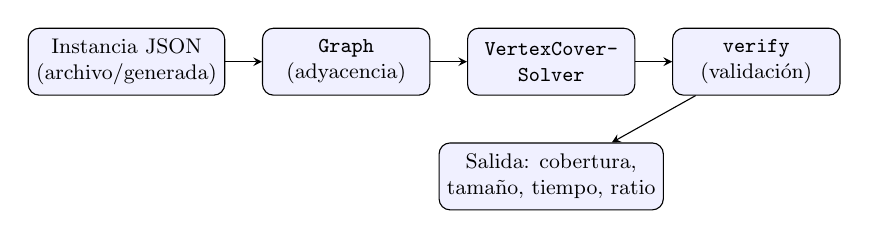
\begin{tikzpicture}[
	scale=0.85, transform shape,
	node distance=0.55cm and 0.55cm,
	box/.style={draw, rounded corners, align=center, minimum width=2.5cm, minimum height=1cm, fill=blue!6, font=\small},
	>=stealth
]
	\node[box] (file) {Instancia JSON\\(archivo/generada)};
	\node[box, right=of file] (graph) {\texttt{\small Graph}\\(adyacencia)};
	\node[box, right=of graph] (solver) {\texttt{\small VertexCover-}\\\texttt{\small Solver}};
	\node[box, right=of solver] (verify) {\texttt{\small verify}\\(validación)};
	\node[box, below=0.7cm of solver] (out) {Salida: cobertura,\\tamaño, tiempo, ratio};

	\draw[->] (file) -- (graph);
	\draw[->] (graph) -- (solver);
	\draw[->] (solver) -- (verify);
	\draw[->] (verify) -- (out);
\end{tikzpicture}
\end{center}

\subsection{Estructura de datos}
Se usa una \textbf{lista de adyacencia} (\texttt{dict[vértice, set[vértice]]}) en lugar de
una matriz de adyacencia:
\begin{itemize}
	\item Las redes reales son dispersas ($|E| \ll |V|^2$), por lo que una matriz
	desperdiciaría memoria: $O(V^2)$ vs. $O(V+E)$ de la lista de adyacencia.
	\item Obtener el grado de un vértice es $O(1)$ (tamaño del conjunto de vecinos),
	operación central en el algoritmo greedy.
	\item Insertar/eliminar una arista es $O(1)$ amortizado gracias al uso de \texttt{set}.
\end{itemize}

\subsection{Formato de archivo de instancia}
Las instancias se guardan en JSON, elegido por ser legible por humanos, nativo en Python y
fácil de versionar en Git (diffs claros por línea):

\begin{lstlisting}
{
  "name": "example_small",
  "description": "...",
  "vertices": ["A", "B", "C", "D", "E", "F"],
  "edges": [["A","B"], ["A","C"], ["A","D"], ["B","C"], ["D","E"], ["E","F"]]
}
\end{lstlisting}

\subsection{Dependencias y decisiones técnicas}
El proyecto depende de \texttt{pytest} (pruebas), \texttt{networkx}, \texttt{matplotlib} y
\texttt{pandas} (candidatas para la Entrega 2, declaradas en \texttt{requirements.txt} pero
aún no integradas al núcleo) y \texttt{pulp} (pendiente de completar su integración). El
núcleo algorítmico (\texttt{src/}) no depende de ninguna librería externa, solo de la
biblioteca estándar de Python, por decisión explícita: mantener el núcleo auditable y sin
puntos de fallo externos, dejando las dependencias externas para capas periféricas
(visualización, experimentación a mayor escala).

% ======================================================
\section{Estrategia de pruebas}
\label{sec:pruebas}

El plan de pruebas está implementado en \texttt{tests/} (27 casos, \texttt{pytest}) y se
organiza en las tres categorías pedidas por la guía:

\begin{center}
\small
\begin{tabular}{p{2.1cm}p{9.3cm}p{2.8cm}}
	\toprule
	\textbf{Categoría} & \textbf{Casos} & \textbf{Archivo} \\
	\midrule
	Básicos    & Construcción del grafo; instancia del Avance 1 (resultado exacto esperado);
	             triángulo $K_3$ (óptimo conocido = 2). & \texttt{test\_graph.py},
	             \texttt{TestCasos\-Basicos} \\[2pt]
	Límite     & Grafo sin aristas; una sola arista (evidencia directa de la cota 2x);
	             vértices aislados; grafo completo $K_4$ (óptimo $=n-1$); componentes
	             desconectadas; fuerza bruta rechazando instancias $>20$ vértices. &
	             \texttt{TestCasos\-Limite} \\[2pt]
	Adversarios & Grafo estrella (greedy óptimo, matching subóptimo pero válido);
	             verificación parametrizada en 10 grafos aleatorios de que el matching
	             maximal nunca supera $2\times$ el óptimo; verificación de que ninguna
	             arista queda sin cubrir. & \texttt{TestCasos\-Adversarios} \\
	\bottomrule
\end{tabular}
\end{center}
\normalsize

\subsection{Criterio de verificación de salidas}
Ninguna prueba confía únicamente en el \emph{tamaño} de la cobertura devuelta. Toda salida
se valida con \texttt{is\_vertex\_cover(graph, cover)} (\texttt{src/verify.py}), que
recorre todas las aristas del grafo y confirma que cada una tenga al menos un extremo en la
cobertura. Esto es intencional: un algoritmo con un error de implementación podría devolver
un conjunto del tamaño "esperado" sin que efectivamente cubra el grafo, y una prueba que
solo comparara tamaños no lo detectaría -- precisamente el tipo de riesgo que produjo el
defecto de reproducibilidad descrito en la Sección~\ref{sec:discusion}.

\subsection{Pruebas de integración y validación cruzada}
Además de las pruebas unitarias por algoritmo, \texttt{TestCasosAdversarios} incluye una
verificación de integración: sobre 10 instancias aleatorias distintas, se ejecutan los tres
algoritmos y se compara el resultado del matching maximal contra el exacto, confirmando que
la cota teórica $|C_{\text{match}}| \leq 2|C^{*}|$ se cumple empíricamente en cada caso, no
solo en la instancia manual del Avance 1.

\subsection{Resultado de la ejecución}
\begin{lstlisting}
$ pytest tests/ -v
...
======================== 27 passed in 0.04s =========================
\end{lstlisting}

% ======================================================
\section{Metodología experimental}
\label{sec:metodologia}

\subsection{Preguntas de evaluación}
\begin{enumerate}[itemsep=2pt]
	\item ¿Qué tan cerca del óptimo queda cada algoritmo aproximado, en la práctica, frente
	a su cota teórica?
	\item ¿Cómo escala el tiempo de ejecución de cada algoritmo con el tamaño de la
	instancia?
	\item ¿A partir de qué tamaño de instancia el algoritmo exacto deja de ser una
	referencia práctica?
\end{enumerate}

\subsection{Hipótesis de trabajo}
Se espera que el greedy por grado obtenga, en promedio, un ratio de aproximación empírico
más cercano a 1.0 que el matching maximal (pese a no tener garantía teórica), y que el
tiempo del algoritmo exacto crezca de forma exponencial con $|V|$, volviéndose impráctico
mucho antes de alcanzar el límite de 20 vértices configurado en el código.

\subsection{Instancias, variables y métricas}
\begin{itemize}
	\item \textbf{Instancias}: grafos aleatorios $G(n,p)$ (modelo Erdős–Rényi), generados
	con la función \texttt{random\_graph} de \texttt{Graph} (archivo \texttt{src/graph.py}),
	con semilla fija por tamaño para reproducibilidad.
	\item \textbf{Variable independiente}: número de vértices
	$n \in \{6, 8, 10, 12, 14, 16, 18\}$, con densidad $p=0.3$ fija en esta primera ronda.
	\item \textbf{Métricas}: tamaño de la cobertura obtenida, ratio de aproximación empírico
	$|C_{\text{algoritmo}}|/|C^{*}|$ (calculado por \texttt{verify.approximation\_ratio}), y
	tiempo de ejecución en milisegundos (\texttt{time.perf\_counter()}).
\end{itemize}

\subsection{Entorno y procedimiento reproducible}
Los experimentos se ejecutan con \texttt{python experiments/compare.py} desde la raíz del
repositorio, sin argumentos ni configuración adicional. El script fija las semillas
aleatorias internamente (\texttt{SEED\_BASE + n}), por lo que una misma ejecución en
cualquier máquina con las dependencias de \texttt{requirements.txt} instaladas debe producir
exactamente los mismos resultados (condición que no se cumplía antes de corregir el defecto
de reproducibilidad de la Sección~\ref{sec:discusion}). El resultado se guarda en
\texttt{experiments/results/comparison.csv}.

% ======================================================
\section{Resultados}
\label{sec:resultados}

\subsection{Validación contra la instancia manual}
Se ejecuta \texttt{demo.py} sobre la instancia \texttt{data/instances/example\_small.json}
(la mini-red de 6 routers de la Sección~\ref{sec:ejemplo-manual}):

\begin{lstlisting}
$ python demo.py --instance data/instances/example_small.json --algorithm all

Cargado: instancia 'data/instances/example_small.json'
  |V| = 6   |E| = 6

[Greedy por grado]
  Cobertura: ['A', 'B', 'E']   Tamano: 3   Valida: SI   Tiempo: 0.034 ms

[Matching maximal (2-aprox)]
  Cobertura: ['A', 'B', 'D', 'E']   Tamano: 4   Valida: SI   Tiempo: 0.018 ms

[Exacto (fuerza bruta)]
  Cobertura: ['A', 'B', 'E']   Tamano: 3   Valida: SI   Tiempo: 0.031 ms

Ratios de aproximacion frente al optimo:
  Greedy por grado: 1.000x
  Matching maximal (2-aprox): 1.333x
\end{lstlisting}

El resultado coincide exactamente con la traza manual de la Sección~\ref{sec:ejemplo-manual},
lo que valida que la implementación respeta el diseño acordado.

\subsection{Experimento comparativo}
Primera corrida del script de experimentos (\texttt{experiments/compare.py}): grafos
aleatorios $G(n, 0.3)$, $n \in \{6, 8, 10, 12, 14, 16, 18\}$, semilla fija por tamaño.

\begin{center}
\begin{tabular}{rrrrrr}
	\toprule
	$n$ & $|E|$ & óptimo & greedy (ratio) & matching (ratio) & $t_{\text{exacto}}$ (ms) \\
	\midrule
	6  & 3  & 2  & 2 (1.00x)  & 4 (2.00x)  & 0.02 \\
	8  & 10 & 4  & 4 (1.00x)  & 6 (1.50x)  & 0.06 \\
	10 & 13 & 5  & 6 (1.20x)  & 10 (2.00x) & 0.31 \\
	12 & 19 & 5  & 5 (1.00x)  & 10 (2.00x) & 0.97 \\
	14 & 35 & 9  & 9 (1.00x)  & 12 (1.33x) & 9.08 \\
	16 & 33 & 9  & 9 (1.00x)  & 14 (1.56x) & 29.61 \\
	18 & 52 & 12 & 12 (1.00x) & 16 (1.33x) & 173.90 \\
	\bottomrule
\end{tabular}
\end{center}

\textbf{Observaciones:}
\begin{itemize}
	\item El tiempo del algoritmo exacto crece de forma visiblemente exponencial incluso en
	este rango pequeño (factor $\approx 6\times$ entre $n{=}16$ y $n{=}18$).
	\item El greedy iguala al óptimo en 6 de las 7 instancias; solo se desvía (ratio 1.2x)
	en $n{=}10$.
	\item El matching maximal se mantiene siempre dentro de su cota teórica (máximo
	observado: 2.0x, exactamente el límite superior), pero nunca superó al greedy en estas
	instancias.
\end{itemize}

% ======================================================
\section{Discusión crítica}
\label{sec:discusion}

\subsection{Interpretación de los resultados frente a la teoría}
Los resultados son consistentes con lo esperado teóricamente: el matching maximal nunca
excedió su cota de $2\times$ el óptimo en ninguna de las instancias probadas (ni en las 7 del
experimento comparativo, ni en las 10 adicionales verificadas automáticamente en
\texttt{TestCasosAdversarios}), lo cual es evidencia empírica -- no una demostración, pero sí
un indicio fuerte -- de que la implementación respeta la garantía demostrada en la
Sección~\ref{sec:diseno-algoritmico}. Que el greedy supere casi siempre al matching maximal
en estas instancias no contradice la teoría: el greedy simplemente carece de una cota
garantizada, lo que significa que \emph{podría} comportarse peor en otras instancias
(por ejemplo, instancias construidas específicamente para explotar su debilidad), no que
sea estrictamente mejor en general. Confirmarlo o refutarlo con instancias adversarias
diseñadas a propósito para el greedy queda como trabajo pendiente para la Entrega 2.

\subsection{El hallazgo del periodo: no determinismo en la implementación inicial}
El hallazgo técnico más relevante de este periodo no aparece en las tablas de resultados,
sino en el proceso: al escribir las pruebas del Avance 2, se detectó que dos ejecuciones
del mismo algoritmo sobre la misma instancia podían devolver coberturas \emph{válidas pero
de tamaño distinto}. La causa raíz, investigada por el grupo, es que Python aleatoriza el
hash de los objetos \texttt{str} entre procesos distintos (\texttt{PYTHONHASHSEED}), por lo
que el orden de iteración de un \texttt{set()} no está garantizado entre ejecuciones. Ambos
algoritmos iteraban directamente sobre conjuntos de aristas, heredando ese no-determinismo.

Esto es importante por dos razones, más allá de ser un simple error de programación: primero,
viola directamente la instrucción adicional 7 de la guía del proyecto ("el repositorio
deberá incluir [...] semillas aleatorias, cuando corresponda" -- la reproducibilidad es un
requisito explícito, no una buena práctica opcional); segundo, sin este arreglo, ningún
resultado experimental de la Sección~\ref{sec:resultados} sería confiable, porque no se
podría distinguir una variación real de desempeño de un simple artefacto de la
aleatorización del hash. Se corrigió introduciendo un orden canónico fijo
(\texttt{\_sorted\_edges}), verificado manualmente variando \texttt{PYTHONHASHSEED} entre
tres valores distintos y confirmando resultados idénticos en los tres casos.

\subsection{Limitaciones y amenazas a la validez}
\begin{itemize}
	\item \textbf{Una sola densidad de grafo.} El experimento comparativo usó únicamente
	$p=0.3$; no se sabe todavía cómo cambian los ratios con grafos más dispersos o más
	densos, ni con topologías distintas a Erdős–Rényi (por ejemplo, la topología tipo
	backbone con hubs de alto grado ya disponible en
	\texttt{data/instances/network\_backbone\_18.json}, generada pero aún no incluida en el
	experimento sistemático).
	\item \textbf{Rango de $n$ limitado por la fuerza bruta.} El óptimo de referencia solo
	se pudo calcular hasta $n=18$ en tiempos razonables; no hay todavía evidencia empírica
	del ratio de aproximación en instancias mayores, donde seguiría siendo necesario el
	solver ILP (pendiente).
	\item \textbf{Una sola corrida por configuración.} Cada punto de la tabla de resultados
	proviene de una única instancia por tamaño (con semilla fija), no de un promedio sobre
	varias instancias del mismo tamaño; el ratio observado para un $n$ dado podría no ser
	representativo de todas las instancias de ese tamaño.
\end{itemize}

\subsection{Cuándo conviene cada alternativa}
Con la evidencia disponible hasta ahora: el \textbf{exacto} solo es viable para instancias
muy pequeñas (en este entorno, claramente impráctico más allá de $n\approx18$-20) y debe
usarse exclusivamente como referencia de validación, nunca en producción. El \textbf{greedy}
es la opción recomendable cuando se prioriza la calidad de la solución sobre la garantía
formal, dado su buen desempeño empírico observado. El \textbf{matching maximal} es
preferible cuando se necesita una \emph{garantía demostrable} sobre el peor caso -- por
ejemplo, en un contexto donde no poder razonar sobre una cota superior sea inaceptable --
incluso a costa de una solución probablemente más grande en la práctica.

% ======================================================
\section{Conclusiones y recomendaciones}
\label{sec:conclusiones}

\subsection{Respuesta a los objetivos}
Los objetivos específicos planteados en la Introducción se cumplieron para el alcance de
esta entrega: el problema está formulado formalmente, el diseño del sistema está
implementado y verificado, se implementaron tres algoritmos (dos más que el mínimo exigido
de dos comparables) con sus garantías demostradas donde corresponde, el plan de pruebas
cubre los tres tipos de casos exigidos con 27 pruebas pasando, el prototipo es ejecutable y
demostrable en vivo, y se ejecutó un primer experimento reproducible con observaciones
documentadas.

\subsection{Síntesis de hallazgos}
El resultado más valioso del periodo no fue un número de la tabla de resultados, sino el
proceso mismo de encontrar y corregir el defecto de reproducibilidad: evidencia directa de
que el plan de pruebas cumple su propósito (detectar errores reales, no solo confirmar lo
esperado) y de que el grupo puede diagnosticar y resolver un problema técnico no trivial sin
supervisión externa.

\subsection{Lecciones aprendidas}
\begin{itemize}
	\item Escribir las pruebas adversarias \emph{antes} de confiar en los resultados
	experimentales permitió detectar un error que un experimento aislado, ejecutado una sola
	vez, nunca habría revelado.
	\item La reproducibilidad no es automática por el solo hecho de fijar una semilla
	aleatoria explícita: estructuras de datos aparentemente inocuas como \texttt{set()}
	pueden introducir no-determinismo oculto si no se tiene cuidado con el orden de
	iteración.
	\item Priorizar el núcleo algorítmico sobre el acabado de las herramientas periféricas
	(como se hizo con la limitación de \LaTeX{}) es consistente con el criterio explícito de
	la guía del proyecto y evitó perder tiempo en un problema no esencial.
\end{itemize}

\subsection{Trabajo futuro (Entrega 2)}
\begin{enumerate}[itemsep=2pt]
	\item Completar e integrar \texttt{exact\_vertex\_cover\_ilp} (PuLP) como referencia
	escalable más allá del límite de la fuerza bruta.
	\item Optimizar \texttt{greedy\_degree\_vertex\_cover} a $O((V+E)\log V)$ con una cola de
	prioridad, verificando con una prueba que ambas versiones produzcan el mismo resultado.
	\item Ampliar la metodología experimental: variar la densidad $p$ además de $n$, e
	incluir instancias tipo backbone (Barabási–Albert), no solo Erdős–Rényi; repetir cada
	configuración sobre varias instancias, no solo una.
	\item Incorporar visualización de grafos pequeños (candidato: NetworkX + matplotlib).
	\item Instrumentar uso de memoria como métrica adicional.
	\item Diseñar instancias adversarias dirigidas específicamente a explotar la falta de
	garantía formal del greedy, para contrastar con el buen desempeño observado hasta ahora.
\end{enumerate}

% ======================================================
\section{Referencias}

\begin{thebibliography}{9}

\bibitem{karp1972}
Karp, R. M. (1972). \emph{Reducibility Among Combinatorial Problems}. En R. E. Miller y
J. W. Thatcher (Eds.), \emph{Complexity of Computer Computations} (pp. 85--103). Plenum
Press.

\bibitem{vazirani2003}
Vazirani, V. V. (2003). \emph{Approximation Algorithms}. Springer-Verlag.

\bibitem{clrs2009}
Cormen, T. H., Leiserson, C. E., Rivest, R. L., \& Stein, C. (2009). \emph{Introduction to
Algorithms} (3.\textsuperscript{a} ed.). MIT Press.

\bibitem{pytest}
pytest documentation. \url{https://docs.pytest.org/}. Consultado en 2026.

\bibitem{pulp}
PuLP documentation -- COIN-OR Foundation. \url{https://coin-or.github.io/pulp/}. Consultado
en 2026.

\bibitem{networkx}
NetworkX documentation. \url{https://networkx.org/documentation/stable/}. Consultado en
2026.

\end{thebibliography}

% ======================================================
\appendix
\section{Anexos}

\subsection{Manual de instalación}
\begin{lstlisting}
git clone <url-del-repositorio>
cd vertex-cover-ids
python3 -m venv venv
source venv/bin/activate        # Windows: venv\Scripts\activate
pip install -r requirements.txt
\end{lstlisting}

\subsection{Manual de uso}
\begin{lstlisting}
# Correr las pruebas
pytest tests/ -v

# Prototipo sobre una instancia conocida
python demo.py --instance data/instances/example_small.json --algorithm all

# Prototipo sobre una instancia nueva generada al vuelo
python demo.py --random 15 0.25 --seed 42 --algorithm all

# Experimento comparativo
python experiments/compare.py
\end{lstlisting}

\subsection{Bitácora de aprendizaje (resumen)}
\label{anexo:bitacora}
El registro completo, con fecha y detalle por sesión, está en
\texttt{docs/bitacora.md} del repositorio. Resumen de las tres sesiones realizadas en este
periodo:

\begin{itemize}
	\item \textbf{Sesión 1}: formulación del problema, formalización de entradas/salidas/
	restricciones, resolución manual de la instancia de ejemplo con ambos algoritmos
	acordados.
	\item \textbf{Sesión 2}: implementación del núcleo (\texttt{Graph}, \texttt{VertexCoverSolver},
	\texttt{verify}), plan de pruebas de 27 casos; hallazgo y corrección del defecto de
	reproducibilidad descrito en la Sección~\ref{sec:discusion}.
	\item \textbf{Sesión 3}: prototipo ejecutable (\texttt{demo.py}), primer experimento
	comparativo reproducible, y documentación de las tres entregas.
\end{itemize}

\subsection{Matriz de contribuciones}
\begin{center}
\begin{tabular}{p{3.2cm}p{10.5cm}}
	\toprule
	\textbf{Integrante} & \textbf{Contribuciones principales} \\
	\midrule
	Integrante 1 & \emph{(completar por el grupo antes de la entrega: módulos, commits y
	pruebas de los que fue responsable)} \\
	Integrante 2 & \emph{(completar)} \\
	Integrante 3 & \emph{(completar)} \\
	Integrante 4 & \emph{(completar)} \\
	\bottomrule
\end{tabular}
\end{center}

\emph{Nota: esta matriz debe completarse con nombres reales y evidencia verificable
(commits de Git, autoría de pruebas o secciones del documento) antes de la presentación,
ya que el atributo AG\_C06 se mide de forma individual aunque el trabajo sea grupal.}

\subsection{Evidencia adicional}
El repositorio Git del proyecto contiene el historial completo de commits, que respalda la
evolución incremental descrita en este informe (estructura inicial → estructura de grafo →
algoritmos → corrección del defecto de reproducibilidad → pruebas → prototipo →
experimento → documentación de cada avance). El resultado crudo del experimento de la
Sección~\ref{sec:resultados} está disponible en
\texttt{experiments/results/comparison.csv}.

\end{document}
